\documentclass[11pt,a4paper]{article}
\usepackage[a4paper,margin=2.35cm]{geometry}
\usepackage{setspace}
\usepackage{graphicx}
\usepackage{booktabs}
\usepackage[numbers]{natbib}
\onehalfspacing
\setlength{\parskip}{0pt}
\setlength{\parindent}{1.15em}
\newcommand{\mfourfigfrac}{0.24}
\newcommand{\mfourpad}{0pt}
\begin{document}

\begin{titlepage}
\centering
\vspace*{24mm}
{\Large Spatial Equity of Walking Access to Public Facilities and Public EV Chargers in Macao SAR\par}
\vspace{1em}
{\large Phase A draft\par}
\vspace{1em}
CS482 Data Science\par
Group X\par
Student ID: Group X\par
\vspace{1em}
20 November 2026\par
\vspace{2em}
\begin{minipage}{\textwidth}
\raggedright
Cross-sectional draft for the 12/03 checkpoint. The cover, references, contribution statement, and AI declaration are outside the main-text page count. Every estimate in the main text is copied from the committed Phase A tables.
\end{minipage}
\end{titlepage}

\section{Introduction}
Residents of Macao do not have the same walking access to parks, public health centres, public libraries, bus stops, and public EV chargers. The research question is descriptive. How unequal is 10-minute and 15-minute pedestrian accessibility across populated H3 cells, and how is zone-level accessibility associated with the share of residents aged 65 or older after accounting for population density?

Three hypotheses were fixed before the estimates were read. H1 says population-weighted accessibility is unequal and spatially clustered. H2 compares the EV Gini with the Gini of parks, health centres, libraries, and bus stops on the same resampled cells. H3 says that, at the scale of the 23 terrestrial census zones, a higher elderly share is associated with lower accessibility once log population density is included. The people who can use the description are planners at DSSCU and DSAT, and residents who want a map of where walking access is thin. The results are correlational and cross-sectional. They do not estimate a causal siting effect, and they are not a build list.

\section{Data Collection and Preparation}
The population layer is the DSEC 2021 census \citep{dsec2021}. Building polygons and statistical zones were read in native EPSG:8433 and transformed to EPSG:32649. The terrestrial control totals are 681,293 residents and 82,751 residents aged 65 or older, after the maritime zone is set aside. Those counts are allocated to H3 cells by area-weighted intersection with the building polygons. The analysis grid has 287 populated resolution-9 cells and 63 populated resolution-8 cells, nested in 23 zones and 7 official parishes, including Taipa.

Public EV chargers come from the CEM map API \citep{cem2026}. Latitude and longitude are swapped to fall inside Macao, and capacity is the number of distinct charger identifiers. Station 9488798 has empty connector records, so its capacity metadata are incomplete and the capacity value 12.0 is imputed from the published pile count. Parks, health centres, libraries, and bus stops are whitelist-filtered against the official SSM, library, and IAM sources and then matched to OpenStreetMap \citep{osm2026}. Deduplication is cross-source only, at 25 m, so opposite bus poles on the same street are kept. The cleaned layer has 240 parks, 11 health centres, 15 libraries, 587 bus stops, and 85 EV charger points.

The walk network is the Geofabrik Macau OpenStreetMap extract \citep{osm2026}. Walking speed is 4.5 km/h. Edges longer than 10 minutes are dropped from the cell graph used later. The network has no slope impedance. Footbridges and overpasses are only those present in OSM, and there is no walkable cross-harbour link, so the Peninsula and the islands stay separate components. Five geographic blocks (seed 42) are frozen for validation. They contain 56 cells with at least one charger. Prevalence is 0.1951. Features for the classifiers are the non-EV whitelist. Columns that start with acc10, acc15, or lisa are excluded, as are the charger target and the charger counts.

\section{Methods}
Accessibility is a Gaussian two-step floating catchment area (2SFCA) score at 10 and 15 minutes \citep{luo2003,dai2010}. Parks, health centres, libraries, and bus stops also form a log-scaled composite index. Inequality is the population-weighted Gini and Theil T, with the convention that zero times the log of zero is zero, plus a within-parish and between-parish split. Uncertainty is a 2000-draw bootstrap, seed 42. Spatial structure uses a global Moran statistic and local indicators of spatial association (LISA) with 999 permutations and Benjamini--Hochberg FDR \citep{anselin1995,bh1995}.

H2 is a paired bootstrap of Gini differences on identical resampled cells, with Holm adjustment across the four traditional facility types. H3 is estimated on the 23 zones, not on the H3 cells, so that building-level allocation is not treated as independent replicates. The pre-specified models are ordinary least squares with HC3 standard errors (OLS), a spatial error model (SEM), and a spatial lag model (SLM). Primary weights are row-standardized $k=4$ nearest neighbours. A bridge-augmented queen matrix is reported beside them. Variance-inflation factors for the two covariates are 1.1585 and 1.1585. A diagnostic p-value is not used to drop or prefer a model. The same Gini, Theil, and Moran summaries are repeated on resolution 8 and resolution 9 as a MAUP check.

The classifier asks only whether a resolution-9 cell currently has a public charger. A constant prior, an L2 logistic regression, and a random forest are scored by spatial-block cross-validation. Imputation and scaling are fit on the training blocks. The reported scores are ROC-AUC, PR-AUC, the Brier score, and the share of positive cells captured in the top fifth of predicted probabilities.

\section{Results}
Figure 1 maps the 15-minute composite surface and the FDR LISA clusters on the 287 cells. Table 1 copies the Gini and Theil intervals, the H3 coefficients, and the out-of-fold scores from the committed outputs.

On resolution-9 cells, the 15-minute EV Gini is 0.4984 (bootstrap interval 0.4315 to 0.5566; Theil T 0.6706). The park Gini is 0.6115, health centres 0.4923, libraries 0.3249, bus stops 0.3876, and the composite Gini is 0.1882 (Theil T 0.0673: 0.0487 within and 0.0185 between parishes). At 10 minutes the EV Gini is 0.5850 and the park Gini is 0.6960. About 35.54 percent of populated cells (1.13 percent of residents) have zero 15-minute EV access. Composite Moran's I is 0.6061 (p 0.0010), with 3 low-low and 9 high-high FDR cells; EV Moran's I is 0.3450 (p 0.0010), with 47 low-low and 1 high-high FDR cells. H1 is supported for both surfaces.

The 15-minute paired difference of EV Gini minus park Gini is -0.1132 (interval -0.1954 to -0.0298; Holm p 0.0550). EV minus library is 0.1734 (Holm p 0.0080) and EV minus bus is 0.1108 (Holm p 0.0080). EV minus health centre is 0.0061 (interval -0.0815 to 0.0936; Holm p 0.8926). Chargers are not uniformly more unequal than every traditional facility. They are more unequal than libraries and bus stops on this grid, and less unequal than parks, with the park contrast sitting next to the Holm threshold. That is an association among historical facility patterns, not a finding that one system was planned more fairly.

For the 15-minute composite on $N=23$ zones, the elderly-share coefficient is 1.9488 under OLS-HC3 (p 0.1400), 1.9366 under SEM, and 1.9635 under SLM. The OLS log-density coefficient is -0.0580. The first OLS-HC3 elderly-share row in the committed file, which is the park outcome, is 3.3187 (p 0.7736). Table 1 places OLS, SEM, and SLM side by side for both outcomes. Under OLS-HC3 the interval covers zero, while spatial ML point estimates are positive (opposite H3's negative direction); H3, as stated, is not supported. The bridge-queen fit is stored alongside and is not used to pick a winner.

The MAUP contrast for the 15-minute composite Gini is 0.2293 at resolution 8 and 0.1882 at resolution 9 (difference -0.0412). The sign and the rough magnitude agree across the two grids. Local Moran values move more than the Gini does, which is the expected scale sensitivity of a cluster statistic.

Out-of-fold ROC-AUC is 0.2171 for the constant prior, 0.8527 for logistic regression (PR-AUC 0.5320, Brier 0.1160, mean fold ROC-AUC 0.7363), and 0.8581 for the random forest (PR-AUC 0.5780, Brier 0.1132, top-fifth hit rate 0.5536, mean fold ROC-AUC 0.7728 with SD 0.1112). The forest and the logistic model are close to each other. Both sit above the constant prior. The gap between the mean fold score and the pooled out-of-fold score is part of the result: the five blocks do not have the same prevalence, so a single pooled ranking is not the same object as the average of within-block rankings.

\begin{center}
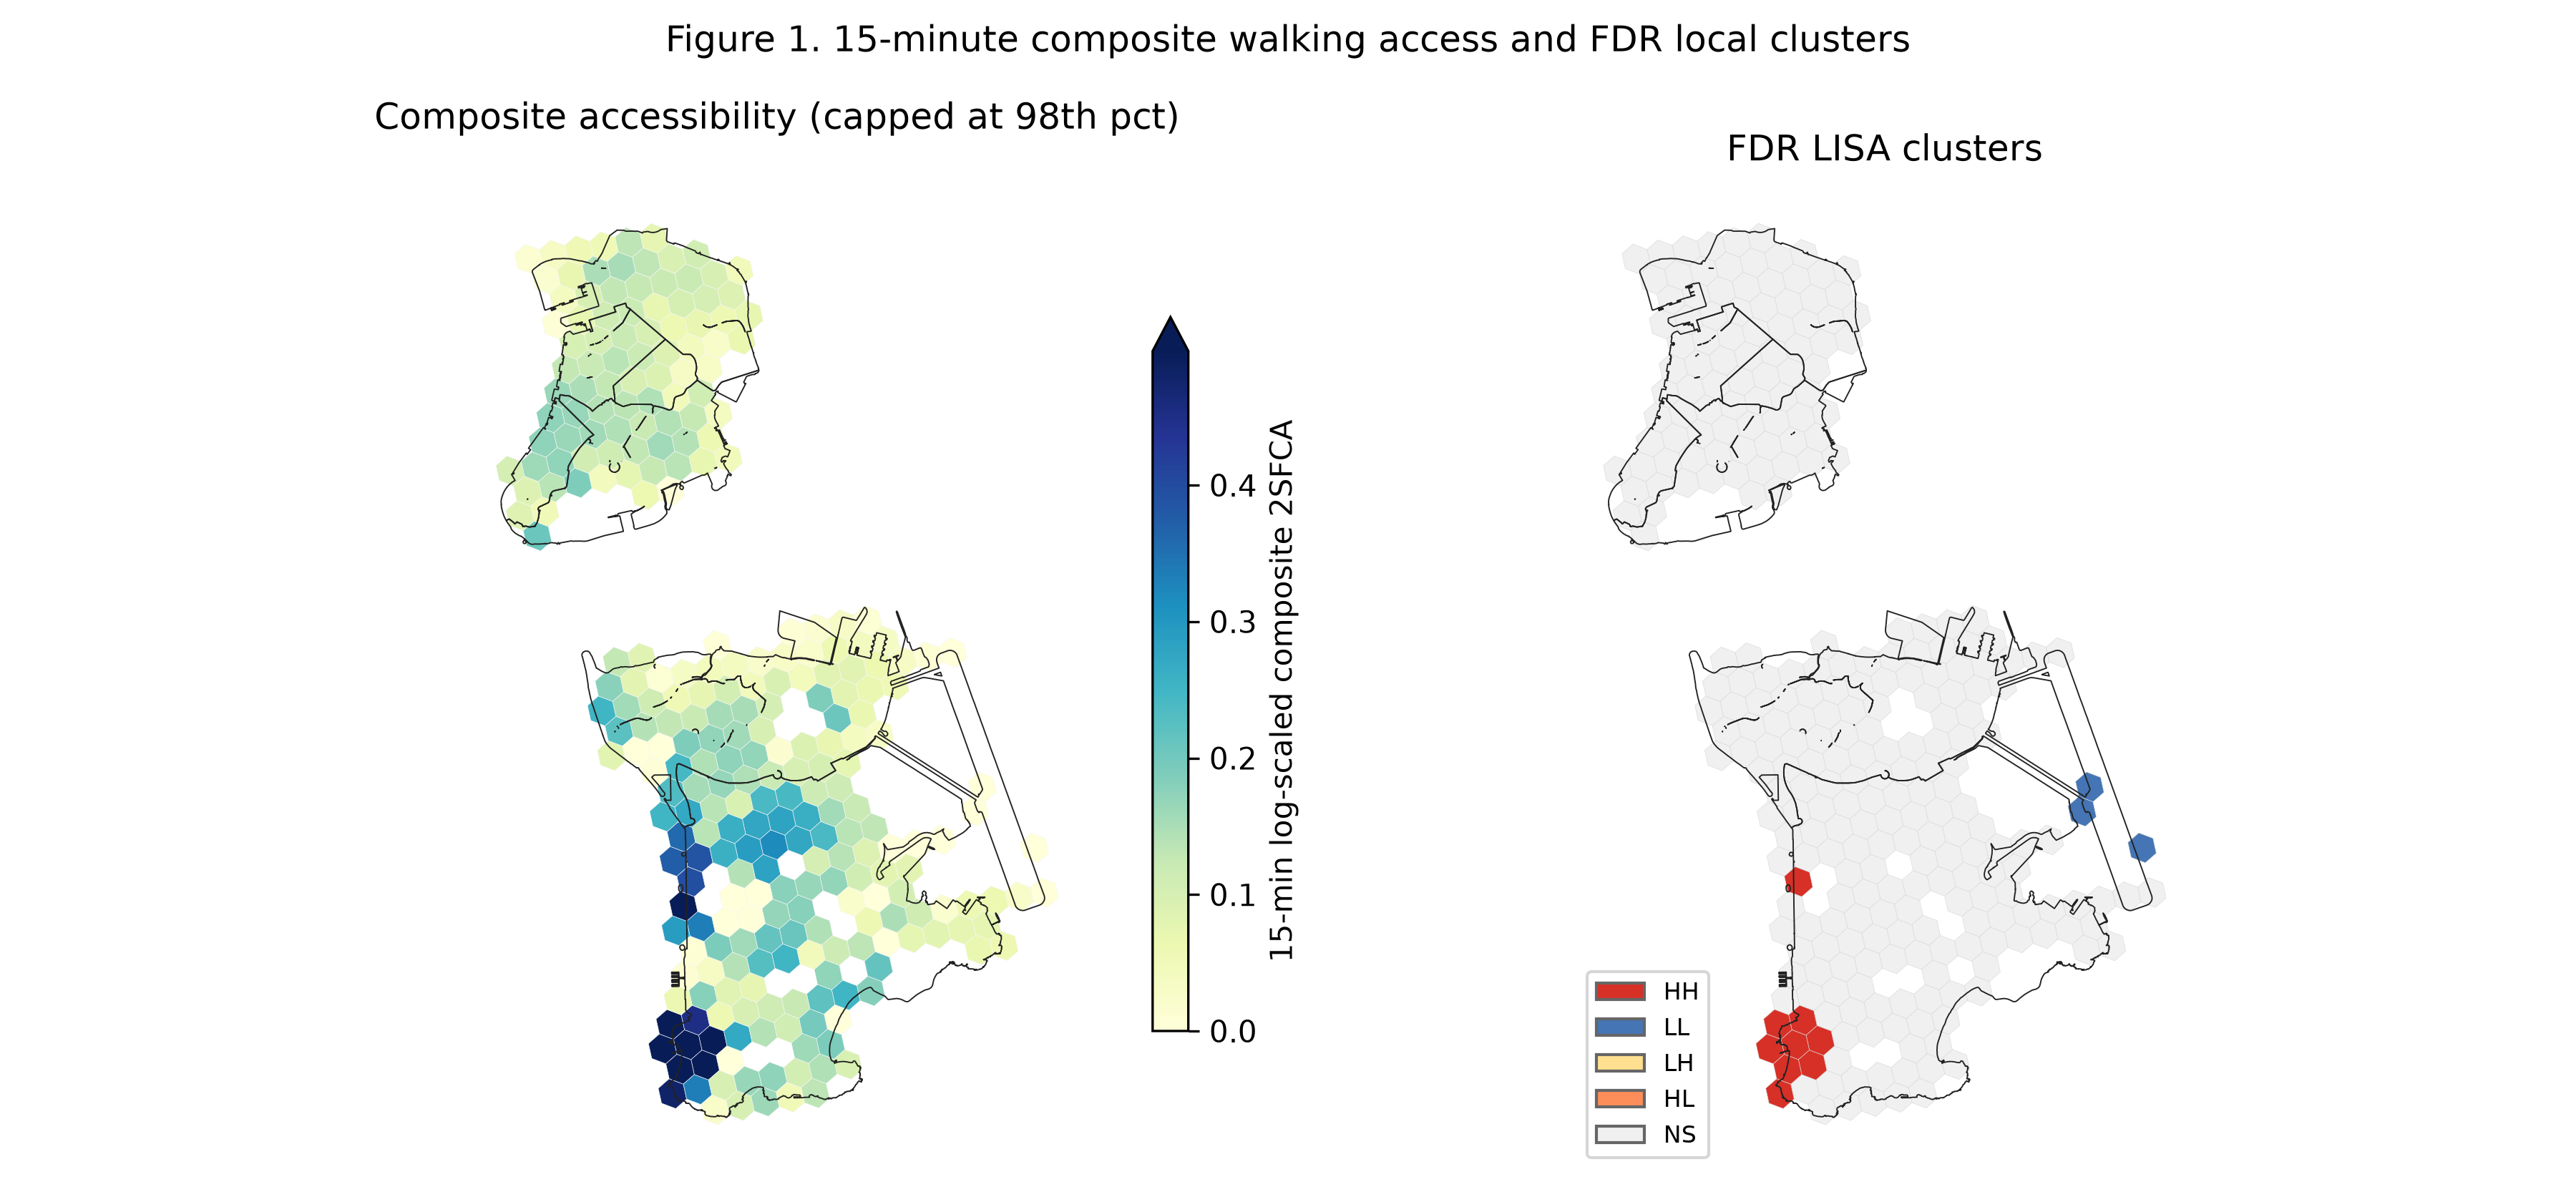
\includegraphics[width=\textwidth,height=\mfourfigfrac\textheight,keepaspectratio]{../outputs/figures/fig1_accessibility_lisa.png}\\[6pt]
{\small Figure 1. Dual panel of 15-minute composite accessibility and FDR LISA clusters. Low-low and high-high colours are the FDR screen, not a siting recommendation.}
\end{center}

\begin{center}
{\small
\textbf{Table 1.} 15-minute Gini and Theil T with bootstrap intervals,
pre-specified H3 elderly-share coefficients, and out-of-fold scores.
OLS, SEM, and SLM stay side by side. A diagnostic p-value does not select a model.
\par\vspace{1em}
\begin{tabular}{lrrrr}
\toprule
Facility & Gini & CI low & CI high & Theil T \\
\midrule
Park & 0.6115 & 0.5288 & 0.6771 & 1.2912 \\
Health centre & 0.4923 & 0.4124 & 0.5655 & 0.5383 \\
Library & 0.3249 & 0.2624 & 0.3920 & 0.2766 \\
Bus stop & 0.3876 & 0.3326 & 0.4411 & 0.5972 \\
EV charger & 0.4984 & 0.4315 & 0.5566 & 0.6706 \\
Composite & 0.1882 & 0.1563 & 0.2202 & 0.0673 \\
\midrule
H3 elderly share & Coef & & & \\
\midrule
Park OLS-HC3 & 3.3187 & & & \\
Park SEM & 2.0076 & & & \\
Park SLM & 3.2136 & & & \\
Composite OLS-HC3 & 1.9488 & & & \\
Composite SEM & 1.9366 & & & \\
Composite SLM & 1.9635 & & & \\
\midrule
Classifier & ROC-AUC & PR-AUC & Brier & \\
\midrule
Constant prior & 0.2171 & 0.1359 & 0.1756 & \\
Logistic regression & 0.8527 & 0.5320 & 0.1160 & \\
Random forest & 0.8581 & 0.5780 & 0.1132 & \\
\bottomrule
\end{tabular}
}
\end{center}


\section{Discussion}
Table 1 answers H1--H3 without a placement rule. Both composite and charger access are unequal and spatially clustered under FDR. Elderly share is not associated with lower zone accessibility in the three pre-specified models. Cells that combine low composite access, no charger, and a high classifier score are candidates for field verification. They record the historical allocation of chargers. They are not sites this study has shown should receive a charger.

Four limitations bound that reading. First, a uniform building-height assumption is not credible in Macao high-rise districts. Building-group counts still leave a dasymetric, building-height error inside one polygon. Second, facility capacity metadata are incomplete: several facilities use unit weights, some park areas are imputed, and station 9488798 uses an imputed capacity of 12.0. Third, walk times ignore slope and topography, miss some footbridges and overpasses, and have no cross-harbour link. Fourth, the ecological fallacy applies: a zone-level association is not an individual association. The reported patterns stay cross-sectional.

\vspace*{\mfourpad}

\bibliographystyle{plainnat}
\bibliography{references}

\section*{Contribution Statement}
This Phase A draft is a group product. The geographic-data role covers census geometries, the CEM feed, the OpenStreetMap walk network, and the H3 grids. The spatial-statistics role covers 2SFCA, Gini, Theil, LISA, and the zone regression. The machine-learning role covers the spatial-block baselines. The remaining role covers the MAUP check, the figures, and the assembly of this draft. Personal names and student numbers are left as Group X until the course roster is attached. No member is credited with a causal siting result.

\section*{AI Usage Declaration}
A coding assistant in Cursor was used for planning, coding, and writing of the Phase A pipeline and of this draft. K-Dense scientific-agent guidance is cited as Kassis and coauthors, arXiv:2609.00065 \citep{kassis2026}. The assistant drafted functions, tests, figure code, and prose. It was not allowed to invent a Gini, a Theil index, a regression coefficient, or an AUC. Verification was a numeric audit that copies each reported figure from the committed CSV or JSON cell, plus unit tests, a frozen-file checksum, and a check that the compiled PDF still contains those same figures. Disagreements were resolved by editing the prose back to the source cell, not by recomputing a new estimate for the sentence.

\end{document}
